\documentclass[11pt,a4paper]{report}

% part of template
\usepackage{url}
\usepackage[utf8]{inputenc}
\usepackage{graphicx}
\usepackage[all]{xypic}
\usepackage{amsmath}
\usepackage{amsthm}
\usepackage{array}
\usepackage{todonotes}
\usepackage{listings}
\usepackage[a4paper]{geometry}

% my packages
% \usepackage{minted}
\usepackage{biblatex}
\addbibresource{bib/thesis.bib}

\def\ci{\perp\!\!\!\perp}
\lstset{language=Python}

\makeatletter %otherwise geometry resets everything
\Gm@restore@org
\makeatother

\setlength{\itemsep}{0cm}
\setlength{\voffset}{0cm}
\setlength{\headheight}{0cm}
\setlength{\topmargin}{0cm}
\setlength{\extrarowheight}{3pt} %for superscripts in tabular
\setlength{\arraycolsep}{4pt}
\lstset{basicstyle = \footnotesize, breaklines = true}

\graphicspath{{imgs/}}

\begin{document}
\begin{titlepage}
\begin{center}
\textsc{\LARGE Bachelor thesis\\Computing Science}\\[1.5cm]

\includegraphics[height=100pt]{logo}

\vspace{0.4cm}
\textsc{\Large Radboud University}\\[1cm]
\hrule
\vspace{0.4cm}
\textbf{\huge Bayesian Constraint-based Causal Discovery with Greedy
  Search}\\[0.4cm]
\hrule
\vspace{2cm}
\begin{minipage}[t]{0.45\textwidth}
\begin{flushleft} \large
\textit{Author:}\\
Daan Spijkers\\
s1011382
\end{flushleft}
\end{minipage}
\begin{minipage}[t]{0.45\textwidth}
\begin{flushright} \large
\textit{First supervisor/assessor:}\\
dr. Tom Claassen \\
\texttt{tomc@cs.ru.nl}\\[1.3cm]
% \textit{[Second supervisor:]}\\
% title, name\\
% \texttt{e-mail adress}\\[1.3cm]
\textit{Second assessor:}\\
title, name\\
\texttt{e-mail adress}
\end{flushright}
\end{minipage}
\vfill
{\large \today}
\end{center}
\end{titlepage}

% The abstract of your thesis is a brief description of the research hypothesis,
% scientific context, motivation, and results.
% The preferred size of an abstract is one paragraph or one page of text.
\begin{abstract}
How much can we improve the accuracy of the resulting PAG from the BCCD
algorithm using a greedy MAG search to optimise its probabilistic causal
statements?
\end{abstract}

\tableofcontents

% The introduction of your bachelor thesis introduces the research area, the
% research hypothesis, and the scientific contributions of your work.
% A good narrative structure is the one suggested by Simon Peyton Jones
% \begin{itemize}
% \item describe the problem / research question
% \item motivate why this problem must be solved
% \item demonstrate that a (new) solution is needed
% \item explain the intuition behind your solution
% \item motivate why / how your solution solves the problem (this is technical)
% \item explain how it compares with related work
% \end{itemize}
% Close the introduction with a paragraph in which the content of the next chapters
% is briefly mentioned (one sentence per chapter).
\chapter{Introduction}\label{introduction}
Causal inference consists of taking a system of statistical
independencies, and mining a system of causal relations. These causal
relations we then represent in a causal graph.

In an ideal situation, we have a statistical test that determines
whether $X$ and $Y$ are independent with 100\% accuracy. Given such a
perfect test, complete algorithms exist; they give the total causal
information possible from that system. Unfortunately, in the real world
100\% accuracy is not possible, and we often have to make do with
insufficient data.

That is why taking realistic data, and optimizing the result is a relevant
problem. It is not always clear how an algorithm performs in these
situations, even if it is complete. One such complete algorithm is
BCCD\cite{claassenBayesianApproachConstraint2012}, which uses a bayesian
score to return a more robust and informative result than comparable
procedures.

BCCD uses a score-based method to mine a system of logical statements of
the following form:
\begin{align*}
  X \Rightarrow Y \lor X \Rightarrow Z \\
  X \not \Rightarrow Y \land X \not \Rightarrow Z
\end{align*}
That is: information about cause or non-cause between different stochastic
variables. These statements have a particular accuracy associated with
them, representing how sure BCCD is about it. BCCD then uses causal
inference to deduce statements that can be mapped into a PAG. However,
since the data can contain inconsistencies, so can the statements. As of
currently, the way inconsistencies are solved is by using statements in
ascending accuracy, thereby never overwriting information we are more sure
of.

However, it is quite possible that one higher accuracy statement, say
$p_1 = 0.9$ is contradicted by two slightly lower accuracy statements,
say $p_2, p_3 = 0.85$. A simple estimation the likelihood of these
situations is:
\begin{align*}
  p_1 * (1 - p_2) * (1 - p_3) &= 0.9 * (1 - 0.85) * (1 - 0.85) &= 0.02 \\
  (1 - p_1) * p_2 * p_3 &= 0.1 * 0.85 * 0.85 &= 0.07
\end{align*}
It is clear then, that we would rather have the second situation, where
the two lower accuracy statements are true, and that there is something to
be gained here.

An initial impulse is to improve the outcome by cleverly choosing which
statements we do use to construct the graph, and which we do not. This
ends up being a very difficult problem however, and instead we will work
the other way around. That is, by starting at the graph.

We take the initial output of BCCD, as well as its logical statements, and
then iteratively search for better graphs until there is no further
improvement possible. Although doing this greedily means this is likely to
end up in a local optimum, the score must end up higher or equal to the
initial BCCD result.

By doing this we will be using global information to complement the local
information, hopefully getting a better result. To easy scoring we will
first convert the BCCD PAG to a MAG, and then work on that MAG. As we will
see, this conversion also improves the result significantly, presumably
because this incorporates global information that the original algorithm
did not.

To summarize, our contributions are as follows:
\begin{enumerate}
  \item An improved result on the BCCD framework by converting to and from
    a MAG.

  \item A greedy step which takes the MAG and BCCD statements, and returns
    a higher scoring MAG.
\end{enumerate}

% This \emph{optional} chapter contains the stuff that your reader needs
% to know in order to understand your work. Your ``audience" consists of
% fellow third year computing science bachelor students who have done the
% same core courses as you have, but not necessarily the same
% specialization, minor, or free electives.
\chapter{Preliminaries}\label{preliminaries}
\section{Causal Discovery by Example}
In this section we will adapt the example given in
\cite{zhangCompletenessOrientationRules2008}, and give a quick
introduction to DAGs and causal discovery in general.

\begin{figure}
  \centering
  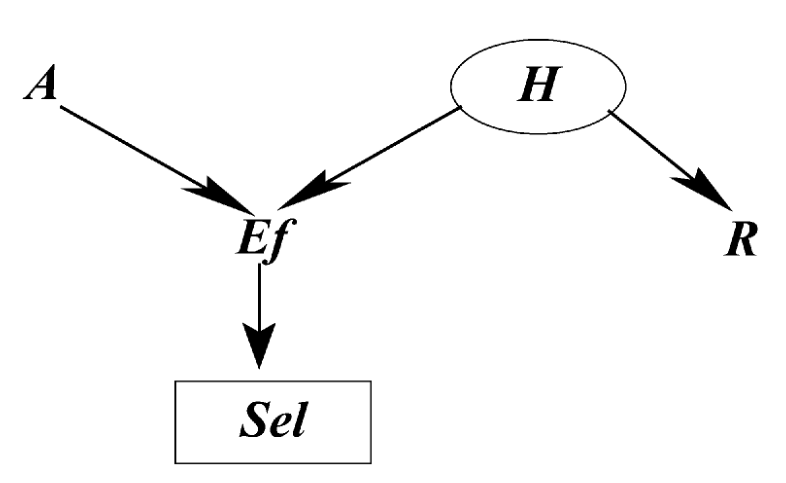
\includegraphics[width=0.5\textwidth]{imgs/example1.png}
  \caption{Example showing both latent cofounders and selection variables.}
  \label{example}
\end{figure}

\section{Ancestral Graphs}

\section{d-seperation}

% This chapter, or series of chapters, delves into all technical details
% that are required to \emph{prove} your scientific hypothesis. It should
% be sufficiently detailed and precise in order for any fellow computing
% scientist student to be able to \emph{repeat} your research and
% therewith establish the same results / conclusions that you have
% obtained. Please note that, in order to improve readability of your
% thesis, you can put a part of this information also in one or more
% appendices (see Appendix \ref{appendix}).
\chapter{Algorithm Overview}\label{algorithm}
Our procedure turns out to be very simple, and we shall see that the most
challenging part is scoring the graph, which we get into in chapter
\ref{problem}. For now we shall give a short overview of the algorithm,
and then go into more detail on each of the problems. We give Python-esque
pseudocode:

\begin{lstlisting}
def bccdgs(pag, statements):
    mag = pag_to_mag(pag)
    next_mag = next_mag(mag)

    while score(next_mag, statements) > score(mag, statements):
      mag = next_mag
      next_mag = next_mag(next_mag)

    return mag_to_pag(mag)
\end{lstlisting}
Where we use one helper function:
\begin{lstlisting}
def next_mag(mag, statements):
    adjacent_mags = adjacent_mags(mag)
    return best_scoring_mag(mags, statements)
\end{lstlisting}
We see that the first thing we do is convert the PAG into a MAG, since
scoring a MAG is easier. Then, within the while loop we keep looking for
the best adjacent mag with the next\_mag function. Within this function we
generate adjacent mags, and then pick the best scoring one. In short,
there are 4 main problems to solve:
\begin{enumerate}
  \item Transforming a PAG into a MAG.

  \item Transforming a MAG into a PAG.

  \item Generating adjacent MAGs.

  \item Scoring a MAG.
\end{enumerate}
We will cover 1-3 in this chapter, and scoring in chapter \ref{problem}.

\section{PAG to MAG}
The main difference is circle marks. The way to do this is by first
orienting all semi-arcs into arcs, and then orienting all remaining edges
into a DAG with no unshielded colliders. See Zhang paper.

\section{MAG to PAG}
Turning a MAG back into a PAG is slightly more involved. We use
d-separation and the FCI orientation rules to do so.

\section{Generating Adjacent MAGs}
This is the simplest problem to solve. We consider adjacent graphs to be
graphs which have one edge changed compared to the original. Given two
vertices $u$ and $v$, there are four possibilities:
\begin{align}
  u \rightarrow v \\
  u \leftarrow v \\
  u \leftrightarrow v\\
  (u, v) \notin E
\end{align}
Remembering that we ignored selection bias, and so there are no undirected
edges. Our original graph has one of these four. All adjacent MAGS can
then be easily generated by adding a graph which has one of the other 3
possibilities.

The real issue comes up when we want to check whether this MAG is also
valid; that is whether it has any almost directed cycles.

\chapter{Logical Statements}\label{problem}
Although we build on the BCCD algorithm, it is quite complex, and details
on how it works are outside of the scope of this thesis. Instead, we will
focus on the specific output we use from it, which is the logical
statements. For the interested reader, we refer to the original paper on
how they are generated\cite{claassenBayesianApproachConstraint2012}.

Given that we ignore selection bias, the specific different logical
statements are as follows:
\begin{align*}
  X &\Rightarrow Y \\
  X \Rightarrow Y &\lor X \Rightarrow Z \\
  X \not \Rightarrow Y &\land X \not \Rightarrow Z \\
  (X, Y) &\notin E \\
  X &\ci Y
\end{align*}
We see that besides information about cause and non-cause, we now also
have information about the non-existence of an edge, and unconditional
independence of variables.

% TODO(daan): figure out how to include pseudocode

\chapter{Results}\label{results}

\section{Nodes}
\begin{figure}
  \centering
  \includegraphics[width=\textwidth]{lib/nodes_causal.pdf}
  \caption{Nodes}
  \label{nodes_causal}
\end{figure}

\section{Graph density}
\begin{figure}[h]
  \centering
  \includegraphics[width=\textwidth]{lib/density_causal.pdf}
  \caption{Density}
  \label{density_causal}
\end{figure}

\section{Skeleton}
\begin{figure}
  \centering
  \includegraphics[width=0.33\textwidth]{lib/skel_causal.pdf}
  \caption{Skeleton}
  \label{skel_causal}
\end{figure}

\section{Cutoff point}
\begin{figure}
  \centering
  \includegraphics[width=0.33\textwidth]{lib/cutoff_causal.pdf}
  \caption{Cutoff}
  \label{cutoff_causal}
\end{figure}

\section{Efficiency}
While the bccd portion, as well as the fci portion are both measured in
seconds, the greedy search is only several miliseconds.

% In this chapter you demonstrate that you are sufficiently aware of the
% state-of-art knowledge of the problem domain that you have investigated
% as well as demonstrating that you have found a \emph{new} solution /
% approach / method.
\chapter{Related Work}\label{relatedwork}
The most notable is
FCI\cite{spirtesCausationPredictionSearch2000}, which is a complete
\cite{zhangCompletenessOrientationRules2008} constrain based algorithm.


% In this chapter you present all conclusions that can be drawn from the
% preceding chapters. It should not introduce new experiments, theories,
% investigations, etc.: these should have been written down earlier in the
% thesis. Therefore, conclusions can be brief and to the point.
\chapter{Conclusions}\label{conclusions}

\printbibliography


% Appendices are \emph{optional} chapters in which you cover additional
% material that is required to support your hypothesis, experiments,
% measurements, conclusions, etc. that would otherwise clutter the
% presentation of your research.
% \appendix
% \chapter{Appendix}\label{appendix}

\end{document}
